\index{dpss@\texttt{dpss}|(}
The \texttt{dpss} library was developed as its own project.  While it is included as part of \texttt{mtpsd}, it can be used separately.

There are two main ways to use the library: the first is through the use of the \code{dpss} class, and the second is to use individual methods that fill user-supplied arrays.

\addtocounter{subsection}{-1}
\subsection{A Note About Taper Lengths}

Recall from Section \ref{sec:dpsscalc} that computing Slepian sequences\index{Slepian sequence|see{DPSS}} involves solving for eigenvectors of a symmetric tridiagonal matrix.  The LAPACK library is used to perform these calculations.  On some machines, LAPACK is only configured by default to handle indices of size \code{INTEGER*2}, which limits the eigenvector length to $2^{16}-1$.  With the splitting technique described in Section \ref{sec:splitting}, this upper-bound can be doubled to $2^{17}-1$.  Longer sequences can only be obtained through interpolation\index{interpolation}. The \code{dpss} class will automatically perform the interpolations if required.

\subsection{Basic Use: the \texttt{dpss} Class}
\index{dpss class@\texttt  {dpss} class|(}

Listing \ref{lst:basicdpss} shows the most basic construction and use of a \code{dpss} object.  
\begin{lstlisting}[label=lst:basicdpss,caption=Basic example of the \texttt{dpss} class]
#include "dpss.h"              /*@\lstomitnum\lstskipnum{8}@*/
...
{
    uint_t n;                   // length of sequences
    double nW;                  // time-bandwidth product   /*@\lstomitnum@*/
    ...                         /*@\lstomitnum\lstskipnum{7}@*/
    
    dpss tapers(n, nW);
    try{
        tapers.compute();       // solves for DPSSs/eigenvalues
    }
    catch(ERR e){
        printf("ERROR: %s\n", e.getmsg());   
    }
    
    printf("h_0(10)=%f, lambda_0=%f \n", tapers(0,10), tapers.lambda(0));    /*@\lstomitnum\lstskipnum{8}@*/
    ...
}
\end{lstlisting} \index{dpss class@\texttt  {dpss} class!compute@\texttt{compute()}}
\smallskip

\noindent In the example, the \code{tapers} object contains the DPSSs and their corresponding energy concentrations.  There are several things to note:
\begin{itemize}
    \item The \code{compute()} method may throw an error of type \code{ERR}\index{ERR class@\texttt{ERR} class} (see Section \ref{sec:simpleerr}).  This error class only has one property: an error message, accessible through \code{ERR::getmsg()}.
    \item All lengths and indices are of type \code{unsigned int}.  A short-form for this type, \code{uint\_t}\index{uint\_t@\texttt{uint\_t}}, is defined in the \code{dpss.h} header.
    \item This basic constructor computes $K=\lfloor2nW\rfloor-1$ data tapers.
    \item If $n>2^{17}-1$, the DPSSs are interpolated from those of length $\tilde{n}=2^{17}-1$ using natural cubic splines.
\end{itemize}
The tapers can then be accessed through one of the accessors described in Table \ref{tbl:dpssaccess}.  The public definition of the \code{dpss} class is given in Listing \ref{lst:dpssclass}.

\index{dpss class@\texttt  {dpss} class!definition|(}
\begin{lstlisting}[label=lst:dpssclass,caption=The \texttt{dpss} class]
class dpss{
    // constructors/destructor
    dpss(uint_t n, double nW);
    dpss(dpss_workspace work);
    ~dpss();

    // computation routines
    void compute();         // computes sequences
    void energize();        // computes eigenvalues

    // accessors
    double operator()(uint_t k, uint_t i);
    double lambda(uint_t k);
    const double* ph();
    const double* pl();
    uint_t length();
    uint_t size(int dim);
    dpss_workspace getinfo();
};
\end{lstlisting}\index{dpss class@\texttt  {dpss} class!definition|)}\index{dpss class@\texttt  {dpss} class!energize@\texttt{energize()}}\index{dpss class@\texttt  {dpss} class!compute@\texttt{compute()}}

\begin{table}[!htb]    
    \caption{ Description of \texttt{dpss} accessors \label{tbl:dpssaccess} \index{dpss class@\texttt{dpss} class!accessors}}
    \vspace*{-0.75em}

    \begin{tabular}{c}
        \hline\hline\\[-0.75em]
        \small
        \parbox{\textwidth-12pt}{
            \vspace*{-0.5em}
            \settowidth{\bodyindent}{\texttt{dpss\_workspacex}}
            \begin{compactcodelist}
                \codeitem{double}{operator()(uint_t k, uint_t i)} Returns $h_k(i)$, the $i$th value of the $k$th DPSS.
                \codeitem{double}{lambda(uint_t k)} Returns $\lambda_k$, the eigenvalue (energy concentration) of the $k$th DPSS.
                \codeitem{double*}{ph()} Returns a pointer to the array of tapers, $h$, so they can be accessed directly.  The tapers are stored as rows of a $K\times n$ array in row-major format.
                \codeitem{double*}{pl()} Returns a pointer to the array of eigenvalues, $\lambda$, so they can be accessed directly.  This array has $K$ elements.
                \codeitem{uint\_t}{length()}  Returns $K\times n$, the total number of elements in the $h$ array.
                \codeitem{uint\_t}{size(int dim)} If \code{dim}=0, returns $n$.  If \code{dim}=1, returns $K$, the number of tapers.
                \codeitem{dpss\_workspace}{getinfo()} Returns a structure that contains all computation parameters used by the \code{dpss} class.
            \end{compactcodelist}
        }\\
        \hline
   \end{tabular}
    \vspace*{-2em}

\end{table}


\subsubsection{The \texttt{dpss\_workspace} Structure}
\index{dpss\_workspace@\texttt{dpss\_workspace}|(}

For more control over the DPSS parameters, a special \code{dpss\_workspace} structure is available.  It's definition is given in Listing \ref{lst:dpsswork}.  The first seven members of the structure specify the computation parameters.  The last one is automatically set by the \code{dpss} class.  The structure has two constructor methods to initialize default values: one takes no inputs, and the other accepts the sequence length and the time-bandwidth product.
\smallskip

\begin{lstlisting}[label=lst:dpsswork,caption=The \texttt{dpss\_workspace} structure]
enum INTERP_TYPE { NONE, LINEAR, SPLINE };

struct dpss_workspace{
    // should be set manually                            [default]
    uint_t n;                    // length of sequence      [0]
    double nW;                   // time half-bandwidth     [1]
    uint_t seql;                 // lower dpss index        [0]
    uint_t sequ;                 // upper dpss index        [2nW-2]
    INTERP_TYPE interp_method;   // interpolation method    [NONE]
    uint_t interp_base;          // interp base length      [n]
    bool energy;                 // if true, compute()      [true]
                                 //    calcs eigenvalues

    // set automatically
    uint_t K;                    //number of sequences
    
    // constructors
    dpss_workspace(): n(0), nW(1), seql(0), sequ(0), K(1), /*@\lstomitnum\lstskipnum{99}@*/
                      interp_method(CALC), interp_base(0), /*@\lstomitnum@*/
                      energy(true) { }                     /*@\lstskipnum{-101}@*/
    dpss_workspace(uint_t n_, double nW_): n(n_), nW(nW_), /*@\lstomitnum\lstskipnum{103}@*/
                      seql(0), sequ(floor(2*nW)-2),        /*@\lstomitnum@*/
                      K(floor(2*nW)-1), interp_method(CALC),/*@\lstomitnum@*/ 
                      interp_base(n_), energy(true) { }    /*@\lstskipnum{-106}@*/
};
\end{lstlisting}
\medskip

Listing \ref{lst:dpssworkexample} shows an example of a workspace being used to initialize a \code{dpss} object.  If any of the supplied parameters are invalid, the \code{dpss} constructor will use the default values.  Alternatively, the \code{dpss\_workspace} can be corrected by supplying it to the function:
\begin{lstplainblock}
void fix_workspace( dpss_workspace &myworkspace ).
\end{lstplainblock}\index{fix\_workspace@\texttt{fix\_workspace()}}
This will directly modify the parameters in the supplied workspace.
\medskip

\begin{lstlisting}[label=lst:dpssworkexample,caption=Example using the \texttt{mtpsd\_workspace} ]
#include "dpss.h"              /*@\lstomitnum@*/
...                             /*@\lstskipnum{8}@*/
{
    dpss_workspace params;

    params.n=pow(2,16);           // sequence length 2^16
    params.nW=3.5;
    params.seql=0;                // lower dpss index
    params.sequ=4;                // upper dpss index
    params.interp_method=SPLINE;  // natural cubic splines
    params.interp_base=pow(2,10)  // interp from 2^10 to 2^16
    params.energy=false;          // don't calculate eigenvalues
                                  //     in compute() method

    dpss tapers(x, params);
    try{
        tapers.compute();         // computes tapers
    }
    catch(...){}                
    tapers.energize();           // Computes eigenvalues using  /*@\label{lst:energize}@*/
                                 //       the interpolated seqs /*@\lstomitnum@*/
    ...                                   /*@\lstskipnum{8}@*/
}
\end{lstlisting}
\index{dpss\_workspace@\texttt{dpss\_workspace}|)}\index{dpss class@\texttt  {dpss} class!energize@\texttt{energize()}}\index{dpss class@\texttt  {dpss} class!compute@\texttt{compute()}}

\subsubsection{Interpolating}
\index{interpolation}

The possible values for \code{interp_method} in the \code{dpss_workspace} are:
\smallskip

{
    \renewcommand{\arraystretch}{1.3}
    \begin{tabular}{ll}
        \code{NONE} & No interpolation\\
        \code{SPLINE} & Interpolate using natural cubic splines\\
        \code{LINEAR} & Linear interpolation
    \end{tabular}
} \smallskip

\noindent If the interpolation method is \code{NONE} but the sequence length is larger than $\hat{n}=2^{17}-1$, then \code{fix_workspace()}\index{fix\_workspace@\texttt{fix\_workspace()}} will change the method to \code{SPLINE} and set \code{interp_base} to $\hat{n}$.  Otherwise, the interpolation base is set to $\min\{$\code{interp_base}, $\hat{n}\}$.

\begin{figure}[!b]
    \centering
    \includegraphics[width=3in]{pics/interp.pdf}
    \caption[Interpolation grid]{Interpolation grid.  \textcolor{green!60!black}{Interior points} are interpolated, but \textcolor{red!70!black}{exterior points} need to be extrapolated using the outer-most splines.\label{fig:interpgrid}}
\end{figure}

For the interpolation routine, the two sequences are assumed to be evaluations of a function at the midpoints of an equally-spaced grid over a common domain.  When interpolating to a larger size, a few points at each end of the sequence must therefore be extrapolated using the outer-most splines.  This idea is depicted in Figure \ref{fig:interpgrid}.  For the natural cubic splines, a zero-derivative boundary condition is assumed at the two end-points.  After the interpolation is performed, the sequences are rescaled to satisfy the unit-energy condition: $\|h_k\|^2 =1$.

In the example in Listing \ref{lst:dpssworkexample}, the \code{dpss} object was set to use natural cubic splines to interpolate from sequences of length $2^{10}$ to sequences of length $2^{16}$.  Since the \code{dpss} class is able to compute sequences of length $2^{16}$ directly, this example allows us to evaluate the interpolation.  With the given parameters, the error norms between the true and interpolated sequences are on the order of  $10^{-5}$ (a 0.001\% error).  This difference is quite small, especially considering that the sequences are expanded by a factor of $64$.  The norms of the errors for both linear and spline interpolated sequences are listed in Table \ref{tbl:interperrors}.

\begin{table}
    \caption[Example interpolation errors]{Interpolation errors for \\$n=2^{16}$, $nW=3.5$, \code{interp_base}=$2^{10}$ \label{tbl:interperrors}}
    \centering
    \renewcommand{\arraystretch}{1.3}
    \vspace*{-0.8em}
    \begin{tabular}{c|rrrrrl}
        \hline\hline
          k & \multicolumn{1}{c}{0} & \multicolumn{1}{c}{1} & \multicolumn{1}{c}{2} & \multicolumn{1}{c}{3} & \multicolumn{1}{c}{4}\\
        \hline
        spline & $5.29$ & $7.40$ & $9.62$ & $10.34$ & $9.40$ & $\times10^{-6}$\\
        linear & $7.79$ & $11.80$ & $14.63$ & $15.64$ & $14.26$ & $\times10^{-6}$\\
        \hline 
    \end{tabular}
\end{table}

\subsubsection{Computing Energy Concentrations}
\index{eigenvalues}

The \code{dpss_workspace} structure has a special member: \code{bool energy}.  If \code{energy} is \code{true}, the \code{dpss::compute()}\index{dpss class@\texttt  {dpss} class!compute@\texttt{compute()}} method will calculate the eigenvalues using Equation \eqref{eq:eigenvalue}.  Otherwise, \code{compute()} will simply set the eigenvalues to a default value of 1.  If you wish to compute the eigenvalues later, the \code{dpss::energize()}\index{dpss class@\texttt  {dpss} class!energize@\texttt{energize()}}\index{dpss class@\texttt  {dpss} class!energize@\texttt{energize()}} method can be called.  This will set the object's \code{energy} property to \code{true}, signaling that computed eigenvalues are available.

There is a subtlety when it comes to determining eigenvalues for interpolated\index{interpolation} sequences.  If \texttt{energy} is \code{true}, the \code{compute()} method will calculate the eigenvalues for sequences of length \code{interp_base}.  These should be close to the eigenvalues for length-$n$ sequences.  This was done to increase speed at little cost in accuracy.  The \code{energize()} method, on the other hand, will force the object to use the sequences of length $n$.

In Listing \ref{lst:dpssworkexample}, the \code{energize()} method was called to force \code{tapers} to use the interpolated sequences when computing the eigenvalues (Line \ref{lst:energize}).  Otherwise, had \code{params.energy} been \code{true}, the values would correspond to sequences of length $2^{10}$.  A comparison of the possible results is given in Table \ref{tbl:interpeigen}.  The eigenvalues for $n=2^{10}$ match those for $n=2^{16}$ to at least six decimal places for $k=0,$ $1$ and $4$.  The eigenvalues for the spline-interpolated sequences, computed with \code{energize()}, match the true values to 11 decimal places, and the linearly-interpolated ones match to 9 decimal places.
\bigskip

\begin{table}[!htb]
    %\caption[Example eigenvalue errors]{Eigenvalues of interpolated sequences\\ $n=2^{16}$, $nW=3.5$, \code{interp_base}=$2^{10}$ \label{tbl:interpeigen}}
    \caption[Example eigenvalue errors]{Eigenvalue results, $n=2^{16}$, $nW=3.5$, \code{interp_base}=$2^{10}$\label{tbl:interpeigen}}    
    \centering
    \renewcommand{\arraystretch}{1.3}
    \vspace*{-0.8em}
    \begin{tabular}{c|ccc}
         \hline\hline
            k &  0 & 1 & 4\\
         \hline
         $n=2^{16}$  & 0.999999993658756               & 0.999999484460341              & 0.993676443756899\\
         $n=2^{10}$  & 0.9999999936\color{red}{61152}  & 0.999999\color{red}{993661152} & 0.993676\color{red}{999048759}\\
          spline  & 0.99999999365875\color{red}{5}  & 0.999999484460\color{red}{287} & 0.99367644375\color{red}{0335}\\
          linear   & 0.99999999365\color{red}{7007}  & 0.9999994844\color{red}{51435} & 0.993676443\color{red}{651266}\\
        \hline
    \end{tabular}
\end{table}
\index{dpss class@\texttt  {dpss} class|)}

\subsection{Advanced Use}

The alternative to using the \code{dpss} class to compute Slepian sequences is to create your own arrays and call methods to fill them.  Unlike the \code{mtpsd} library, some of these methods do create workspace arrays on the heap.  Brief descriptions of the advanced methods are given in the following sections.  A list and description of the common variables, needed by several of the procedures, is given in Table \ref{tbl:dpsscommonvars}.

\begin{table}
    \centering
    \caption{Common variables in the \texttt{dpss} library \label{tbl:dpsscommonvars}}
    \renewcommand\arraystretch{1.3}
    \vspace*{-1.5ex}
    \small
    \begin{tabular}{r@{\hspace{1.5ex}}p{5ex}@{\hspace{2ex}}p{0.65\textwidth}}
        \hline\hline
        \code{uint\_t} & \code{n} & the length of the discrete prolate spheroidal sequences.\\
        \code{double} & \code{nW} & the time-bandwidth product of the sequences.\\
        \code{double*} & \code{h} & pointer to the array containing the DPSSs, stored as rows in row-major format.  \code{h} has length $K\times n$.\\
        \code{double*} & \code{l} & pointer to the array containing the eigenvalues (energy concentrations).  \code{l} has length $K$.\\
        \code{uint\_t} & \code{seql} & the index of the first DPSS in \code{h}.  This value is usually zero, indicating the first computed DPSS is $h_0$.\\
        \code{uint\_t} & \code{sequ} & the index of the last DPSS in \code{h}.  \code{h} contains all sequences $h_\text{seql}$ to $h_\text{sequ}$.\\
        \code{uint\_t} & \code{K} & the total number of sequences in \code{h}\\
        \hline
    \end{tabular}
\end{table}

\subsubsection{Computing Eigenvectors}
\index{eigenvectors}

In order to compute eigenvectors, the publicly available LAPACK library is used.  A few routines have been written to interface with LAPACK, which automatically build the necessary workspace arrays.
\medskip

\begin{lstshortblock}
void eig_rrr(uint_t n, double *D, double *E, uint_t il, uint_t iu, 
             double *eig_val, double *eig_vec, uint_t vec_length)
void eig_rrr(uint_t n, double *D, double *E, uint_t il, uint_t iu, 
             double *eig_val, double *eig_vec)
\end{lstshortblock}\index{eig\_rrr@\texttt{eig\_rrr()}}
\begin{fdescription}
    Inputs: & \code{n, D, E, il, iu, (vec_length)}\\
    Outputs:& \code{eig_val, eig_vec}\\
    Workspace: & \code{uint\_t[10*n+2*K]}, \code{double[20*n]}\\
    & Computes the eigenvectors/eigenvalues of a symmetric tridiagonal matrix using LAPACK's Relatively Robust Representations method (\code{dstevr\_}).  The error tolerance is set to the machine's safe minimum (\code{dlamch\_}).  \code{D} and \code{E} are arrays containing the diagonal and off-diagonal elements, respectively, of the \code{n}$\times$\code{n} tridiagonal matrix.  The indices \code{il} and \code{iu} are the lower and upper eigenvalues to compute, where eigenvalues are arranged in increasing order beginning with index 1.  \code{vec_length} is the distance between the first elements of consecutive eigenvectors.  \code{eig\_val} and \code{eig\_vec} are pointers to the output eigenvalue and eigenvector arrays.  This routine may throw an error of type \code{LAPACK_ERROR()}\index{LAPACK_ERROR class@\texttt{LAPACK\_ERROR} class} if LAPACK fails (see Section \ref{sec:simpleerr}).
\end{fdescription}\index{eig\_rrr@\texttt{eig\_rrr()}}
\fdbottom
\vspace*{-1.5em}

\begin{lstshortblock}
void eig_iit(uint_t n, double *D, double *E, uint_t il, uint_t iu, 
             double *eig_val, double *eig_vec, uint_t vec_length)
void eig_iit(uint_t n, double *D, double *E, uint_t il, uint_t iu, 
             double *eig_val, double *eig_vec)
\end{lstshortblock}
\begin{fdescription}
    Inputs: & \code{n, D, E, il, iu, (vec_length)}\\
    Outputs:& \code{eig_val, eig_vec}\\
    Workspace: & \code{uint\_t[5*n+K]}, \code{double[5*n]}\\
    & Computes the eigenvectors and eigenvalues of a symmetric tridiagonal matrix using LAPACK's bisection and inverse iteration methods (\code{dstebz_}/\code{dstein\_}).  The error tolerance is set to the machine's safe minimum (\code{dlamch\_}).  \code{D} and \code{E} are arrays containing the diagonal and off-diagonal elements, respectively,  of the \code{n}$\times$\code{n} tridiagonal matrix.  The indices \code{il} and \code{iu} are the lower and upper eigenvalues to compute, where eigenvalues are arranged in increasing order and begin with index 1.  \code{vec_length} is the space between the first elements of consecutive eigenvectors.  \code{eig\_val} and \code{eig\_vec} are pointers to the output eigenvalue and eigenvector arrays.  This routine may throw an error of type \code{LAPACK_ERROR()} if LAPACK fails (see Section \ref{sec:simpleerr}).
\end{fdescription}\index{eig\_iit@\texttt{eig\_iit()}}
\fdbottom

\noindent The two previous methods perform the same operation, but use different LAPACK routines.  The relatively robust representations method is faster, but requires a larger workspace.  The inverse iteration method uses less memory and is supposedly more accurate, but is slower.  The \code{vec_length} term allows for additional space between computed eigenvectors.  This is useful for the splitting technique, where only the first half of each eigenvector is computed.  The second halves are filled later based on symmetry.

\subsubsection{Computing the DPSSs}

\begin{lstshortblock}
void dpss_calc(uint_t n, double nW, int seql, int sequ, double *h)
void dpss_calc(uint_t n, double nW, int seql, int sequ, 
               void (*eig_calc)(uint_t n,double* D,double* E, 
                               uint_t il, uint_t lu, double* eig_vec, 
                               double* eig_val, uint_t vec_length), 
               double *h)
\end{lstshortblock}
\begin{fdescription}
    Inputs: & \code{n, nW, seql, sequ, (eig_calc)}\\
    Outputs: & \code{h}\\
    Workspace: & \code{double[n+2]} + \texttt{eig\_calc} workspace\\
    & Computes the discrete prolate spheroidal sequences $h_\text{seql}$ to $h_\text{sequ}$ using the symmetric tridiagonal method with even-odd splitting (Section \ref{sec:splitting}).  The optional \code{eig_calc} is a pointer to the function that computes eigenvectors.  This must have the same form as \code{eig_rrr()} and \code{eig_iit()} described previously.  If no eigenvalue routine is provide, \code{eig_iit()} is used.
\end{fdescription}\index{dpss\_calc@\texttt{dpss\_calc()}}
\fdbottom
\vspace{-2em}
\pagebreak

\noindent Eigenvectors are only unique up to a scaling factor.  When an eigenvector is normalized, its magnitude is fixed, but it may still have one of two polarizations: $+v$ or $-v$.  Thus, a polarization convention is needed.
\medskip

\begin{lstshortblock}
void normalize_vec(double *h, uint_t n)
\end{lstshortblock}
\begin{fdescription}
    Inputs: & \code{h, n}\\
    Outputs: & \code{h}\\
    & Scales \code{h} to have a unit norm.
\end{fdescription}\index{normalize\_vec@\texttt{normalize\_vec()}}
\medskip

\begin{lstshortblock}
void polarize_dpss(double *h, uint_t n, uint_t k)
\end{lstshortblock}
\begin{fdescription}
    Inputs: & \code{h, n, k}\\
    Outputs: & \code{h}\\
    & Orients \code{h}$_\text{k}$ so that even sequences have a positive mean, and odd sequences satisfy:  $\;\sum (n-1-2i)\,h_\text{odd}(i)>0$.  Note that here, \code{h} is a single sequence of length \code{n}.  The index \code{k} is only used to check if the sequence is even or odd.
\end{fdescription}\index{polarize_dpss@\texttt{polarize\_dpss()}}
\fdbottom

\noindent The \code{dpss_calc()} routine automatically scales and polarizes the sequences.

\subsubsection{Interpolating}
\index{interpolation}

The following two methods can be used to interpolate from one number of points to another.  It is assumed that the two arrays correspond to the centre values of an equally-spaced grid over a common domain, as shown in Figure \ref{fig:interpgrid}.
\medskip

\begin{lstshortblock}
void linear_interp( double *y, uint_t n, uint_t nout, double *z )
\end{lstshortblock}
\begin{fdescription}
    Inputs: & \code{nout, y, n}\\
    Outputs: & \code{z}\\
    Workspace: & \code{double[n]}\\
    & Linearly interpolates \code{y} from \code{n} points to \code{nout} points.  The result is stored in \code{z}.  A local copy of \code{y} is made, so it is safe to have \code{y=z}.
\end{fdescription}\index{linear_interp@\texttt{linear\_interp()}}
\medskip

\begin{lstshortblock}
void spline_interp( double *y, uint_t n, uint_t nout, double *z)
\end{lstshortblock}
\begin{fdescription}
    Inputs: & \code{y, n, nout}\\
    Outputs: & \code{z}\\
    Workspace: & \code{double[2*n]}\\
    & Interpolates \code{y} from \code{n} points to \code{nout} points using natural cubic splines.  A zero-derivative boundary condition is used for the outer splines.  The result is stored in \code{z}.  It is safe to have \code{y=z}.
\end{fdescription}\index{spline_interp@\texttt{spline\_interp()}}
\fdbottom

\subsubsection{Computing Energy Concentrations}
\index{eigenvalues}

Energy concentrations are computed using Equation \eqref{eq:eigenvalue}, which is only useful for discrete prolate spheroidal sequences.  If a custom taper is supplied, the value returned will not necessarily represent the true concentration of energy for $f\in[-W,W]$. 
\smallskip

\begin{lstshortblock}
extern void compute_energy_concentrations( double *h,uint_t n, uint_t K, 
                                           double nW, double *l )
\end{lstshortblock}
\begin{fdescription}
    Inputs: & \code{h, n, K, nW}\\
    Outputs: & \code{l}\\
    Workspace: & \code{double[2*n]}, \code{fftw\_complex[2*n+2]},  (without FFTW: \code{double[n]})\\
    & Uses an external routine to compute the energy concentrations of tapers in \code{h}, and stores the results in \code{l}.
\end{fdescription}\index{compute_energy_concentrations@\texttt{compute\_energy\_concentrations()}}
\fdbottom

\noindent The method is declared as \code{extern} because the code is in one of two separate files: either \texttt{dpss\_fftw.cpp} or \texttt{dpss\_nofftw.cpp}.  In \texttt{dpss\_fftw.cpp}, the FFTW3 library is used to compute $\lambda$ in Equation \eqref{eq:eigenvalue}, exploiting the Toeplitz nature of the matrix $A$.  In \texttt{dpss\_nofftw.cpp}, the required matrix-vector multiplication is done with loops.  The \texttt{fftw} version requires $6\times$ the amount of working memory, but the improvement in speed is extreme.  It is advised to use the \texttt{fftw} version, which is compiled into the library by default.  The \texttt{nofftw} source is included, however, if you wish to build it manually as a replacement.

\subsubsection{An Advanced Example}

The following example uses spline interpolation to compute discrete prolate spheroidal sequences of length $10^7$.  A plot of the resulting sequences is shown in Figure \ref{fig:dpssadvanced}.  Notice how on Line \ref{lst:dpssfilltail}, the initial DPSS computation (length $2^{16}$) fills the tail end of \code{h}.  This was done so the interpolation step on Line \ref{lst:dpssinterp} would not overwrite any sequences.
\smallskip

\begin{lstlisting}[label=lst:dpssadvanced,caption=A \texttt{dpss} advanced example ]
#include "dpss.h"              /*@\lstomitnum@*/
...                             /*@\lstskipnum{8}@*/
{
    // parameters
    uint_t n = pow(10,7);           // dpss length 10^7
    uint_t nb = pow(2,16);          // interp base length 2^16
    uint_t nW = 2.5;
    uint_t seql = 1;                // starts at h1 (not h0)
    uint_t sequ = 5;
    uint_t K = sequ-seql+1;
    uint_t istart=n*K-nb*K;         // start filling h here    

    // allocate memory
    double *h = new double[n*K];    // tapers
    double *l = new double[K];      // eigenvalues

    // calculate base size sequences using 
    //       eig_iit for eigenvectors/values
    // NOTE: tail of h is filled, allowing for 
    //       interpolation without overwriting
    try{
        dpss_calc( nb, nW, seql, sequ, &eig_iit, &h[istart] ); /*@\label{lst:dpssfilltail}@*/
    } 
    catch( ERR e ){
        printf("Error: %s", e.getmsg());
        return;
    }
    
    // interpolate and re-normalize
    for (uint_t ii=0; ii<K; ii++){
        spline_interp(&h[istart + ii*nb], nb, n, &h[ii*n]); /*@\label{lst:dpssinterp}@*/
        normalize_vec( &h[ii*n], n);
    }

    // compute energy concentrations
    compute_energy_concentrations(h, n, K, nW, l);  /*@\lstskipnum{7}\lstomitnum@*/
    ...                                             /*@\lstomitnum@*/

    // cleanup
    delete [] h;    delete [] l;
}
\end{lstlisting}\index{eig\_rrr@\texttt{eig\_rrr()}}\index{dpss\_calc@\texttt{dpss\_calc()}}\index{spline_interp@\texttt{spline\_interp()}}\index{normalize\_vec@\texttt{normalize\_vec()}}\index{compute_energy_concentrations@\texttt{compute\_energy\_concentrations()}}
\medskip

\begin{figure}[!hb]
    \centering
    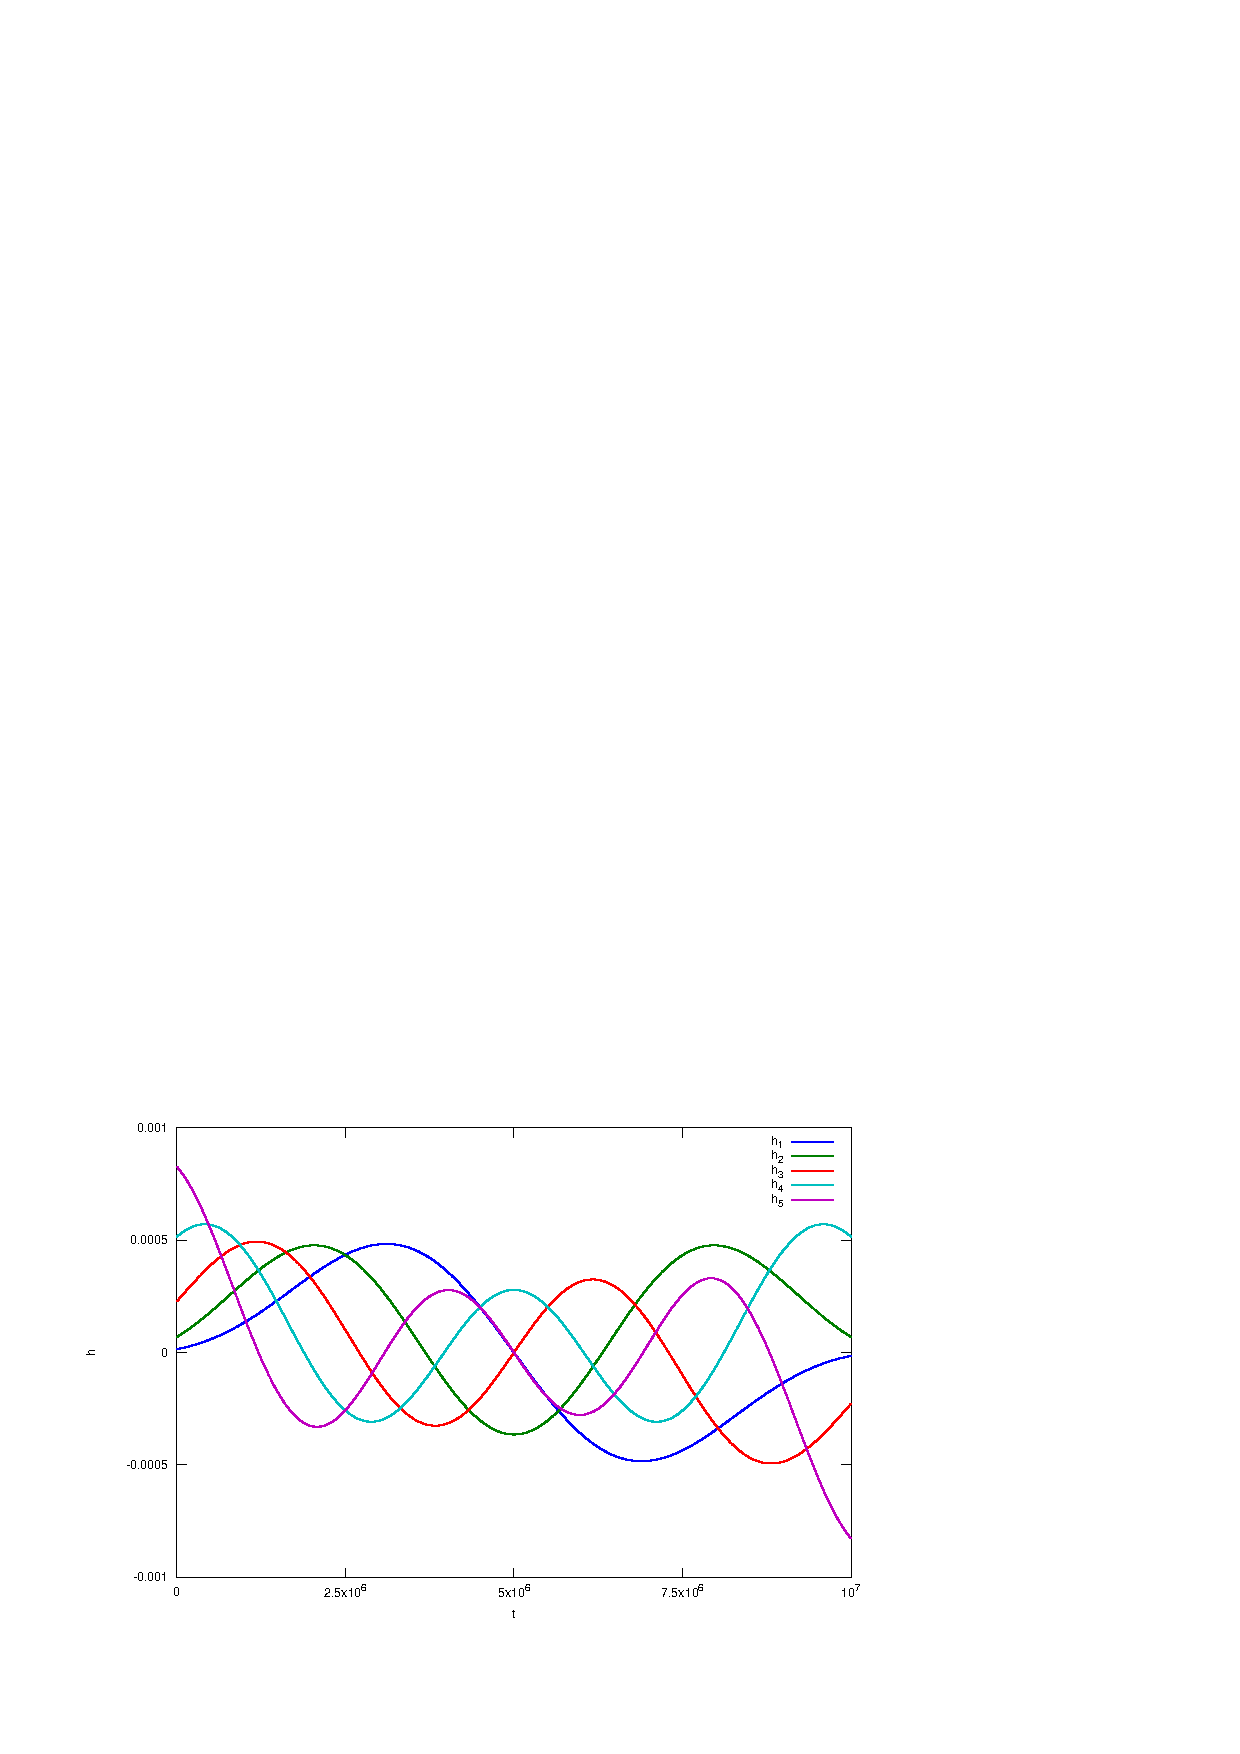
\includegraphics[width=0.9\textwidth]{pics/dpss1e+07.pdf}
    \vspace*{-0.5em}

    \caption[Advanced DPSS Example]{Discrete prolate spheroidal sequences computed in Listing \ref{lst:dpssadvanced}.\label{fig:dpssadvanced}}
    \vspace*{-0.5in}
\end{figure}

\index{dpss@\texttt{dpss}|)}